\documentclass{report}
\usepackage{outline}

% [outline] includes new outline environment. I. A. 1. a. (1) (a)
% use \begin{outline} \item ... \end{outline}
\usepackage{subfig}
\usepackage{graphicx}
\usepackage{times}
\usepackage{epstopdf}
\usepackage{amsmath}
\usepackage[utf8]{inputenc}
\usepackage[T1]{fontenc}
\usepackage{mathtools}
\usepackage{multirow}
\usepackage{float}
\usepackage{hyphenat}
\usepackage{color} 
\usepackage{fancyhdr}
 
\pagestyle{fancy}
\fancyhf{}
\rhead{OpenFF Group}
\lhead{Bayesian Inference Parameterization Manuscript Outline}
\rfoot{Page \thepage}

\newcommand{\cov}[1] {\mathrm{cov}\left( #1 \right)}
\newcommand{\var}[1] {\mathrm{var}\left( #1 \right)}


\title{Outline: Bayesian sampling driven classical mechanics force field parameterization}
\author{Bryce C. Manubay}
\date{\today}
\begin{document}
{\let\newpage\relax\maketitle}
\begin{outline}
  \item{Objective: Test and validate use of Bayesian sampling driven parameterization procedure using inexpensively generated single molecule simulation data 
        as experimental evidence}
  \item{Intro:}
  \begin{outline}
    \item{Classical mechanics simulations have been useful in the study of chemistry, biology and materials ranging from the simple to very complex. However 
          the force fields that scientists use in their studies aren’t always consistent and an element of uncertainty to any study done.}
    \begin{outline}
      \item{Produce quantitatively different results depending on the force field \cite{ffcomp1,ffcomp2,ewen_comparison_2016,petrov_are_2014,
            guvench_comparison_2008}}            
      \item{Can make choice of force field more important than it should be}
    \end{outline}
    \item{Current force field parameterization efforts are heuristic and often guided by the physical intuition of scientists rather than systematically.
          \cite{parm94,tip3p,tip4pew,burger,law,combined,rational,aipar}
    \begin{outline}
      \item{Go through cited examples explicitly}
      \item{ForceBalance: tries to be somewhat more quantitative by minimizing an objective function.  However, weights are still chosen by hand. 
            [more discussion]\cite{FB1,FB2,FB3}}
      \item{Find more examples}
    \end{outline}
    \item{Big reason behind this being how force fields are optimized to reproduce very specific types of “target data”\cite{unchanged,monticelli}}
    \begin{outline}
      \item{There is no single right way to optimize a force field to reproduce all kinds of observables}
      \begin{outline}
        \item{Usually, when you optimize for certain observables, estimates of other observables can become less accurate}
      \end{outline}
      \item{Additionally, it is difficult to update existing force fields with new kinds of data (either more molecular diversity or new properties) without 
            changing the entire force field}
      \begin{outline}
        \item{Forcefield parameters are inherently coupled by nature of how they are designed (sometimes weakly, sometimes strongly)}
        \item{Chemically/physically, interactions and geometries at an atomic scale are coupled}
        \item{You often need to adjust all (or many) parameters if you adjust one}
        \item{Could be a lot, could be a little. Situations vary depending on how the changing interactions affect the overall system}
      \end{outline}
      \item{\bf We would like to probabilistically determine all FAMILIES of force fields consistent with given data in a systematic manner. Also, given more 
            data (new data), we would like a method  to update extant force fields, so that new force fields could be determined to given this new data.}
    \end{outline}
    \item{Bayesian statistics has been applied to a large number of big data and optimization problems \cite{bayes1,bayes2,bayes3,bayes4,bayes5,bayes6,bayes7,
          bayes8}}
    \begin{outline}
      \item{add citations from the recent lit stuff on OpenFF Slack}
    \end{outline}
    \item{With this in mind the authors of this paper have developed a novel process for parameterizing classical mechanics force fields using experimental 
          data as evidence for Bayesian inference driven parameterization. For this particular paper we have set up a toy case in order to test and validate 
          the Bayesian inference parameterization.}
    \begin{outline}
      \item{The experimental data used as evidence will be trajectory data produced from a force field developed by members of our force field 
            parameterization team.\cite{smirff}}
      \item{For simplicity and time considerations the simulated data is only of single molecules and hence the parameters being changed will be limited to 
            those involved in bonded interactions. Specifically:}
      \begin{outline}
        \item{bonded force constants}
        \item{equilibrium bond lengths}
        \item{angular force constants}
        \item{equilibrium bond angles}
        \item{torsional force constants} 
      \end{outline}
      \item{We will investigate if the Bayesian inference approach will recover the original force field parameters using the simulated data under the original
            force field as evidence if the force field is perturbed.}
    \end{outline}
  \end{outline}
  \item{Methods}
  \begin{outline}
    \item{Molecules?}
    \begin{outline}
      \item{$\leq 3$ carbons}
      \item{$\leq 2$ oxygens}
    
      \begin{figure}[h!]
      \centering
  
      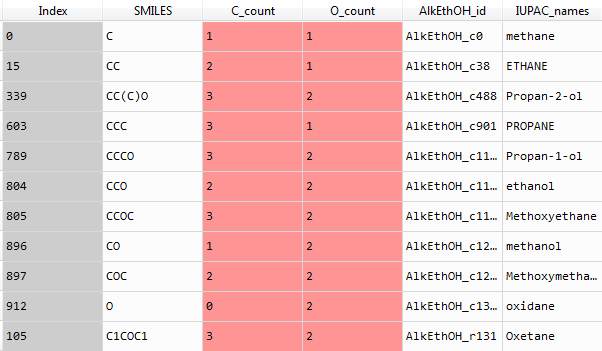
\includegraphics[width=.9\linewidth]{bayes1_mols.PNG}
      \label{fig:sub1}
      \caption{The molecules being used as the test set for this initial parameterization. Each row entry includes the SMILES string, C and O composition, 
               ID from the AlkEthOH set and the IUPAC name for a given molecule.}
      \end{figure}
    \end{outline}
    \item{Simulations}
    \begin{outline}
      \item{Generate simulation data by simulating a set of AlkEthOH molecules using the ‘smirff99Frosst’ forcefield}
      \item{Simulation parameters:}
      \begin{outline}
        \item{Thermostated to 300 K}
        \item{0.5 ns time steps}
        \item{Friction coefficient of 1 ps$^{-1}$}
        \item{4 ns simulations}
        \item{Frame recored every 1000 steps}
      \end{outline}
      \item{Currently making O-H LJ parameters small and finite in order to keep hydrogens from floating into other atoms}
    \end{outline}
    \item{Sampling the Bayesian Posterior}
    \begin{outline}
      \item{Observables:}
      \begin{outline}
        \item{Bonds and Angles:}
        \begin{outline}
          \item{It is well known that simulated bond and angle frequency distributions can be well described by simple gaussian distributions}
          \item{We therefore choose observables to be simple parameters of the gaussian distribution}
          \begin{outline}
            \item{Mean bond lengths and angles}
            \item{Variance of bond lengths and angles}
          \end{outline}
        \end{outline}
        \item{Torsions:}
        \begin{outline}
          \item{Torsion distributions are generally more difficult to describe than bonds and angles}
          \item{Additionally, distributions are often multimodal and may not have constant period between modes}
          \item{Hence, we choose to describe torsion distributions as fourier series expansions of the form:}
          \begin{outline}
            \item{$f_{N}\left(x\right) = \sum_{i=0}^N A_i \sin^2\left(\frac{2 i \pi x}{\tau_i} + \psi_i \right)$}
            \item{Fourier series coefficients, phase angles, and periodicities will be the observables used to describe the distributions}
          \end{outline}
        \end{outline}
      \end{outline}
      \item{Bayes' Theorem}
      \begin{outline}
        \item{Simple version: $Pr\left(\Theta|O\right) = \frac{Pr\left(O|\Theta\right)Pr\left(\Theta\right)}{Pr\left(B\right)}$}
        \item{Where $Pr\left(\right)$ is a probability function and $\Theta$ are parameters for a model estimating our observed data $O$}
      \end{outline}
      \item{Prior probability models}
      \begin{outline}
        \item{Simple uniform priors for all parameters}
        \item{Limits on uniforms dependent on parameter}
        \begin{outline}
          \item{Equilibriun bond lengths and angles: $\pm 20\%$ of the true parameter value}
          \item{Force constants: 0 as the floor and twice the highest value in the force field as a ceiling}
          \begin{outline}
            \item{Bonded force constant: 0 to 4000 $\left(\frac{kcal}{mol \cdot \AA^2}\right)$}
            \item{Angular force constant: 0 to 1400 $\left(\frac{kcal}{mol \cdot rad^2}\right)$}
            \item{Torsional force constant: 0 to 21 $\left(\frac{kcal}{mol}\right)$}
          \end{outline}
        \end{outline}
      \end{outline}
      \item{Liklihood function}
      \begin{outline} 
        \item{Forward models have already been determined and are simple (how do we calculate bond lengths and angles from a time series of coordinates?)}
        \begin{outline}
          \item{Bond Length}
          \begin{outline}
            \item{$r_{i,j} = \sqrt{\left(\bar{x}_i - \bar{x}_j\right)^2}$}
            \item{where $r_{i,j}$ is the bond length between atoms i and j and $\bar{x}_i$ are the atomic coordinates of atom i}
          \end{outline}
          \item{Bond Angle}
          \begin{outline}
            \item{$\dot{x}_{i,j,k} = \left(\bar{x}_i - \bar{x}_j\right) \cdot \left(\bar{x}_j - \bar{x}_k\right)$
            \item{$\theta_{i,j,k} = \arccos \frac{\dot{x}_{i,j,k}}{r_{i,j} \cdot r_{j,k}}$}
            \item{where $\theta_{i,j,k}$ is the angle between bonded atoms i,j and k}
          \end{outline}
          \item{Torsion Angle}
          \begin{outline}
            \item{$\hat{x}_{i,j} = \frac{\left(\bar{x}_i - \bar{x}_j\right)}{\sqrt{\left(\bar{x}_i - \bar{x}_j\right)^2}}$}
            \item{$n_{i,j,k} = \hat{x}_{i,j} \times \hat{x}_{j,k}$}
            \item{$m = n_k \times \hat{x}_{i,j}$}
            \item{$y = n_{i,j,k} \cdot n_{j,k,l}$}
            \item{$z = m \cdot n_{j,k,l}$}
            \item{$\phi_{i,j,k,l} = \arctan \frac{y}{z}$}
            \item{where $\phi_{i,j,k,l}$ is the torsion angle formed by atoms i,j,k and l}
          \end{outline}
        \end{outline}
        \item{There are a few possible options for choices of likelihood functions}
        \begin{outline}
          \item{$L\left(O|\Theta\right) = \frac{1}{\sqrt{2\pi\sigma_O^2}} \cdot \exp\left(-\frac{\left(\bar{O} - O_{mod}\left(\Theta\right)\right)^2}{2
                   \sigma_O^2}\right)$}
          \item{$L\left(O|\Theta\right) = \prod_{j=1}^M \frac{1}{\sqrt{2\pi\sigma_O^2}} \cdot \exp\left(-\frac{\left(O_j - O_{mod}\left(\Theta\right)
                  \right)^2}{2\sigma_O^2}\right)$}
          \item{$L\left(O|\Theta\right) = \exp\left(-\frac{\frac{1}{M} \sum_{j=1}^M \left(O_{mod}\left(\Theta\right) - O_j\right)^2}{2\sigma_O^2}\right)$}
        \end{outline}
      \end{outline}
      \item{Sampling and choice of surrogate model}
      \begin{outline}
        \item{What is a surrogate model?}
        \begin{outline}
          \item{Surrogate models allow us to inexpensively determine outcomes that cannot be easily measured directly}
          \item{In the context of our force field parameterization, we use surrogate models to estimate simulated observables cheaply in order to 
		  inexpensively sample our posterior}
          \item{Surrogate models can allow us to accelerate posterior sampling and by updating the model frequently (as more data is available) provide an 
                  accurate final answer}
          \item{**Currently looking up best practices for making accurate surrogate models with sparse high dimensional data}
          \item{Will use lowest level of complexity possible here (like splining for example)}
        \end{outline}
      \end{outline}
      \item{Multistate reweighting using MBAR}
      \begin{outline}
        \item{Not too sure how useful this is going to be if we can use surrogate modeling to help assess likelihood instead}
        \item{Maybe just demonstrate surrogate modeling vs. using MBAR to help speed sampling on smaller scale?}
        \item{Utility of MBAR}
        \begin{outline}
          \item{Way more efficient than direct simulation}
          \item{Able to describe parameters of estimated distribution when there is significant configurational overlap with the original}
        \end{outline}
        \item{Utilized in the same way surrogate modeling would be, but less efficient (we think)}
        \item{Preliminary results have shown that reweighting with MBAR is accurate within conservative changes of $3\%$ in bonded force constant and $2\%$
                change in minimum bond length. Thus, each move during posterior construction will end in a new simulation on that cusp to generate new 
                evidence before the next reweighting move.}
      \end{outline}
      \item{Proposing new parameter states and MCMC acceptance criteria}
      \begin{outline}
        \item{Every iteration of the MCMC sampling procedure a new set of parameters are proposed based on the current state and a prescribed proposal width.
              Right now that is done by randomly sampling from a normal distribution where the current parameter value is the average and the proposal width is
              the standard deviation of the normal distribution}
%MRS: which normal distribution?  Do you mean this is a user-defined parameter?  I think in this case, once we have O(theta), then any reasonable strategy is fine.  If we were doing the sampling with direct simulation, we would want as accurate as possible, but for the surrogate model, pretty much anything would work.
        \item{During a single iteration of the sampling loop we calculate the likelihood and prior probabilities of both the current and the proposed parameter
%MRS: can you define ``the sampling loop'' here? (perhaps referring to a specific outline bullet point?)
              states. The acceptance probability ($p_{accept}$) is the ratio of the proposal probability to the current probability ($\frac{L_{current} 
              Pr_{current}}{L_{proposal} Pr_{proposal}}$). If the acceptance probability is greater than a random sample generated on $Uniform\left(0,1\right)$
              then we accept the proposed state and update our position (i.e. the proposed state becomes the current state). A new iteration now begins.
        \item{If the acceptance criteria are not met then the current state is retained, a new move is proposed  and the cycle is repeated.}
%MRS: hmm.  are you just defining metropolis MC (with Gaussian probability definitions?)
      \end{outline} 
      \item{Proposed MCMC sampling algorithm and experiments}
      \begin{outline}
        \item{\textit{Hypothesis:} The speed of convergence of the sampling is affected by the order and frequency by which surrogate modelling and MBAR are utilized to predict observable quantities in place of classical mechanics simulations.} 
        \begin{outline}
          \item{\textbf{Step 1:} Simulate with an altered force field prescribed by the initial parameter states which are an input to the sampler function or 
                those proposed by the last step of the sampler.}
%MRS: agreed.
          \item{\textbf{Step 2:} Calculate the observables associated with the parameters being changed (bond length average and variance for bonded parameter 
                types, bond angle average and variance for angle parameter types, etc.)}
%MRS: agreed.
          \item{\textbf{Step 3:} Several options are possible in step 3, in order to test our hypothesis}
%MRS: Important that this is not the main hypothesis, but a subsidiary one.  We basically have three flavors of sampling: direct sampling, MBAR, and surrogate models -- with a number of parameters for each. for MBAR, we have ``how far out in each parameter is reasonable to go''? For surrogate models, we have a gigantic family of models to choose from (which we have to sort out - eventually, though we really only need to find one that works)
          \begin{outline}
            \item{\textbf{3a:} Use MBAR to conservatively extend our knowledge of the observables in local parameter space. From this 
%MRS: more specifically, from this local knowledge of O(\theta)
we can construct 
                  surrogate models for the observables and carry out MCMC sampling on the surrogate models. 
%MRS: well MCMC sampling to perform bayesian inference using the surrogate models as the data forward map.
Once the sampling has converged (which can be
                  heuristically determined by examining the previous few MCMC samples), carry out a new simulation at that final state.}
%MRS: probably not just previous 'few' MCMC samples, since we need to know the distribution is converging.
%MRS: below -- can you be a bit moe detailed on 3b and 3c?  Try to make it clear enough so that someone who was knowledgeable about the area but wasn't in our conversations (say David Mobley) could actually carry out the process.
            \item{\textbf{3b:} Repeat steps 1 and 2 N more times (prescribed parameter states determined by MCMC acceptance criteria) and then use those N+1
                  simulations to construct surrogate models for our observables. Carry out MCMC sampling on the surrogate models. Once the sampling has 
                  converged, carry out a new simulation at that final state.}
            \item{\textbf{3c:} Same as 3b, but without the use of MBAR.}
          \end{outline} 
          \item{\textbf{Step 4:} Carry out a new simulation with parameters prescribed by a new proposed MCMC move and calculate the observables associated 
                with the parameters being changed. If the calculated observables are statistically the same as those from the previous parameter state then
                the sampling has fully converged and the final parameters have been determined. Else, go back to step 1.} 
        \end{outline} 
      \end{outline}   
    \end{outline}
  \end{outline}
      
  \item{Results and Analyses}
  \begin{outline}
    \item{Ideas for deliverables/presentation of results:}
    \begin{outline}
      \item{I think it would be worthwhile to show the evolution of the posterior distribution over iterations, so maybe show a few snapshots of 
                the posterior heat map for select SMIRKS (k vs x$_0$, or the equivalent for the angle parameters) over iterations, i.e.  
      \begin{figure}[h!]
      \centering
  
      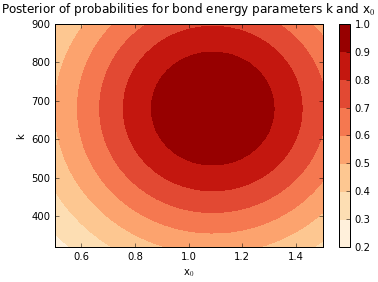
\includegraphics[width=.9\linewidth]{fake_post.PNG}
      \label{fig:sub1}
      \caption{Final iteration of 2D heatmap representation of posterior probability distribution marginalized over all others.}
      \end{figure}
      \item{Show any non-gaussian posteriors}
      \item{Want to compare our final Bayesian sampled forcefield to the original}
      \begin{outline}
        \item{How different are they?}
        \item{Compare observables}
        \item{Error}
        \item{Confidence intervals on final parameter values pulled from posterior (need to investigate best way to go about this)}
      \end{outline}
      \item{Efficiency of process with and without surrogate modeling (just simulation vs with MBAR vs with surrogate modeling)}
    \end{outline}
  \end{outline}
  \item{Conclusions}
  \begin{outline}
    \item{Impacts of study and implication for uses of classical force field parameterization}
    \item{Highlight that, despite practical complexity, the parameterization process can and will get much more complex}
    \item{We have presented a novel and fully automated process for parameterization of classical force fields driven by Bayesian inference given some 
              experimental data. Not only does the process provide fully automated parameter optimization and selection based on probability, but also a 
              means to update extant classical force fields with new experimental data. The original force field parameters were all recovered within 
              the uncertainties that we determined from their posterior distributions (let's assume). 
    \item{While we have only presented a toy problem to test the validity and efficiency of the process; we have well demonstrated the challenges 
              presented by force field parameterization. Moreover, we have shown that using simple surrogate models in order to cheaply calculate 
              observables a function of parameter greatly decreases the costs of assessing the likelihood function. While this was not imperative to 
              the success of this initial parameterization problem, it will be as we move towards using bulk phase properties as evidence where large 
              scale simulations will become a prohibitive computational expense when assessing the likelihood function.}     
  \end{outline} 
\end{outline}       
\bibliographystyle{ieeetr}
\bibliography{bayes1_manuscript}
\end{document}
